%%% use twocolumn and 10pt options with the asme2e format
\documentclass[twocolumn,10pt]{asme2e}
\special{papersize=8.5in,11in}


%%% Packages
\usepackage{nameref}
\usepackage{lipsum}% http://ctan.org/pkg/lipsum
\usepackage{multirow}
\usepackage{graphicx}% Include figure files
\usepackage{dcolumn}% Align table columns on decimal point
\usepackage{bm}% bold math
\usepackage{newtxtext}
\usepackage[utf8]{inputenc}
\usepackage[T1]{fontenc}
\usepackage{mathtools}
\usepackage{mathrsfs}
\usepackage{amsmath, amssymb}
\usepackage[dvipsnames]{xcolor}
\usepackage{color}

\graphicspath{{Figures/}}
%Added commands
\newcommand{\todo}[1]{{\textcolor{Red}{\bf[[Todo: #1]]}}}




\confshortname{IDETC/CIE 2021}
\conffullname{the ASME 2021\\ International Design Engineering Technical Conferences \&\\
              Computers and Information in Engineering Conference}

\confdate{August 17--21}
\confyear{2021}
\confcity{Virtual}
\confcountry{Online}

%%% Replace DETC2009/MESA-12345 with the number supplied to you 
%%% by ASME for your paper.
%<<<<<<< HEAD
\papernum{DETC2021-XXXXX}
%=======
\papernum{DETC2021/VIB-XXXXX}
%>>>>>>> fcf48567cfddc0253a6ce281f9fdf7074a3dd825

%%% You need to remove 'DRAFT: ' in the title for the final submitted version.
\title{Guidelines for Optimizing the error in area ratio damping estimation method}

%%% first author
\author{Balija Santoshkumar\thanks{Address all correspondence to this author.}
    \affiliation{
	Department of Mechanical Engineering\\
	Michigan State University\\
	East Lansing, Michigan 48824\\
    Email: balijasa@msu.edu
    }	
}

%%% second author
%%% remove the following entry for single author papers
%%% add more entries for additional authors
\author{Firas A.~Khasawneh 
    \affiliation{
	Department of Mechanical Engineering\\
	Michigan State University\\
	East Lansing, Michigan 48824\\
    Email: khasawn3@egr.msu.edu
    }
}

\begin{document}

\maketitle    

%%%%%%%%%%%%%%%%%%%%%%%%%%%%%%%%%%%%%%%%%%%%%%%%%%%%%%%%%%%%%%%%%%%%%%
\begin{abstract}
  %!TEX root = ..\arxiv_Dampinguncertanity_manuscript.tex
%-------------------------------
%*******************************
The logarithmic decrement (log-dec) is one of the most popular methods for viscous damping estimation in linear, single degree of freedom systems. 
It estimates the damping ratio by examining the decay in the amplitude between two peaks some number of cycles apart. 
The accuracy in the estimation is sensitive to the chosen number of cycles, where the latter can be optimized such that the uncertainty in the estimation is minimized. 
However, the log-dec method is not suitable for systems with high damping ratios (approximately $>0.3$).  
Another recent approach for damping estimation is based on considering a ratio of the amplitudes of the positive and negative areas in the free response of the oscillator. 
Although prior works on the areas method only tested lightly damped systems, we show here that---in contrast to log-dec---this approach can estimate the damping ratio over the whole range of underdamped linear oscillators. 
However, in contrast to log-dec, there are no available guidelines on how many areas to include in the damping estimation. 
In this work, we derive uncertainty analysis expressions for the areas method and we utilize them to obtain the optimal number of areas to use. 
Our results show that for a very low damping ratio ($<0.01$), choosing more than two areas in the estimation increases the uncertainty. 
In contrast, for moderate to high damping (between $0.05$ and $1$), we need to consider all the available areas in the estimation. 
One caveat in the range of high damping (between $0.3$ and $1$) is that while it is desirable to include all the available areas, uncertainty increases when considering up to 3 areas. 
Therefore, if only 4 areas are available in this range, then to reduce the uncertainty in the estimate only the first two areas must be considered. 
The results are verified using a large number of numerical simulations including different levels of noise. 
\end{abstract}
%%%%%%%%%%%%%%%%%%%%%%%%%%%%%%%%%%%%%%%%%%%%%%%%%%%%%%%%%%%%%%%%%%%%%%
%!TEX root = ..\arxiv_Dampinguncertanity_manuscript.tex
%-------------------------------
%*******************************
\section{INTRODUCTION} \label{sec:intro}
Damping estimation is a critical attribute to predict accurate dynamics of the system. There are several well-established methods to predict the damping in an oscillatory system. One of the well-known methods is logarithmic decrement~\cite{1890a}, which is initially developed for determining the viscosity of the fluids. Now, it is widely used in estimating the damping in structures~\cite{Fang1996}, cantilever beams~\cite{Liao2011}, plates~\cite{Saito1982}, wind turbines~\cite{Hansen2006}, and energy harvesters~\cite{Stanton2010}. The other methods of damping estimation are random decrement technique~\cite{Ibrahim1977}, weighted response-integral method~\cite{GAYLARD2001}, wavelet transforms~\cite{Ahmed2016}. Fang-LinHuang et al. (2007)~\cite{Huang2007} proposed a new method for identifying structural damping, which overcomes the limitations of the logarithmic decrement method. This method gives a better estimation of damping in noisy signals with a high damping ratio compared with the logarithmic method.

Recently, J A. Little \& B P. Mann~\cite{Little2019} derived an analytical expression for the optimal no of periods to be considered in the logarithmic decrement method to minimize the error in the predicted damping. Uncertainty analysis is performed to arrive at the optimal no of periods. In this paper, we develop guidelines to pick the optimal number of areas to be considered in Fang-LinHuang et al. (2007)~\cite{Huang2007} work. We perform uncertainty analysis to develop the guidelines. The new method for identifying structural damping~\cite{Huang2007} gives better results than the logarithmic decrement method, and we develop guidelines to pick the optimal no of periods to make this approach even more robust in estimating the damping ratio.

The subsequent sections of this work as follows. First, we give the background about minimizing the error in the logarithmic decrement method. Next, we perform the uncertainty analysis approach to the area ratio damping estimation method. We also perform a large number of numerical simulations to arrive at the optimal number of areas to be considered. We conclude with results of minimizing the error in the area ratio damping estimation method.
%%%%%%%%%%%%%%%%%%%%%%%%%%%%%%%%%%%%%%%%%%%%%%%%%%%%%%%%%%%%%%%%%%%%%%
%!TEX root = ..\arxiv_Dampinguncertanity_manuscript.tex
%-------------------------------
%*******************************
\section{BACKGROUND}
\label{sec:background}
%*******************************
We consider a single degree of freedom oscillatory system with viscous damping as
\begin{equation}
\ddot{x}+2 \xi \omega_{n} \dot{x}+\omega_{n}^{2} x=0,
\end{equation}
where $x$, $\dot{x}$ and $\ddot{x}$ are the oscillator displacement, velocity and acceleration respectively. $\xi$ is the damping ratio, $\omega_{n}$ is the natural frequency of the system.
The response of the system is given by
\begin{equation}
x(t)=A \mathrm{e}^{-\xi \omega_{n} t} \sin \left(\omega_{d} t+\varphi\right),
\end{equation}
where $\omega_{d}=\omega_{n} \sqrt{1-\xi^{2}}$, $A$ and $\varphi$ are determined by initial conditions.
From the logarithmic decrement method we know the damping ratio of a system with exponential decay is given by
\begin{equation}
\label{eqn1}
\xi=\frac{\delta}{\sqrt{\delta^{2}+4 \pi^{2}}},
\end{equation}
where $\delta=\frac{\ln \left(\frac{x_{0}}{x_{N}}\right)}{N}$ is the logarithmic decrement, $x_{0}$ is the magnitude of the first sample, and $x_{N}$ is the magnitude of the sample $N$ periods later.

Applying error propagation to Eq.~\ref{eqn1} gives the uncertainty in estimated damping $U(\xi)$ is related to uncertainty in the measurements $U_{x}$ by

\begin{equation}
\label{eq2}
U^{2}_{\xi}=\left[\left(\frac{\partial \xi}{\partial x_{0}}\right)^{2}+\left(\frac{\partial \xi}{\partial x_{N}}\right)^{2}\right] U_{x}^{2},
\end{equation}
evaluating Eq.~\ref{eq2} gives us

\begin{equation}
U^{2}_{\xi}=\frac{1}{4} \frac{\pi^{4}\left(-\xi^{2}+1\right)^{3}}{N^{2}\left(\pi^{2} \xi^{2}+\left(-\xi^{2}+1\right) \pi^{2}\right)^{3}}
\left( 1+\left(\frac{N \pi \zeta}{\mathrm{e}^{\sqrt{-\zeta^{2}+1}}}\right)^{2} \right) U_{x}^2.
\end{equation}
\begin{figure*}[h]



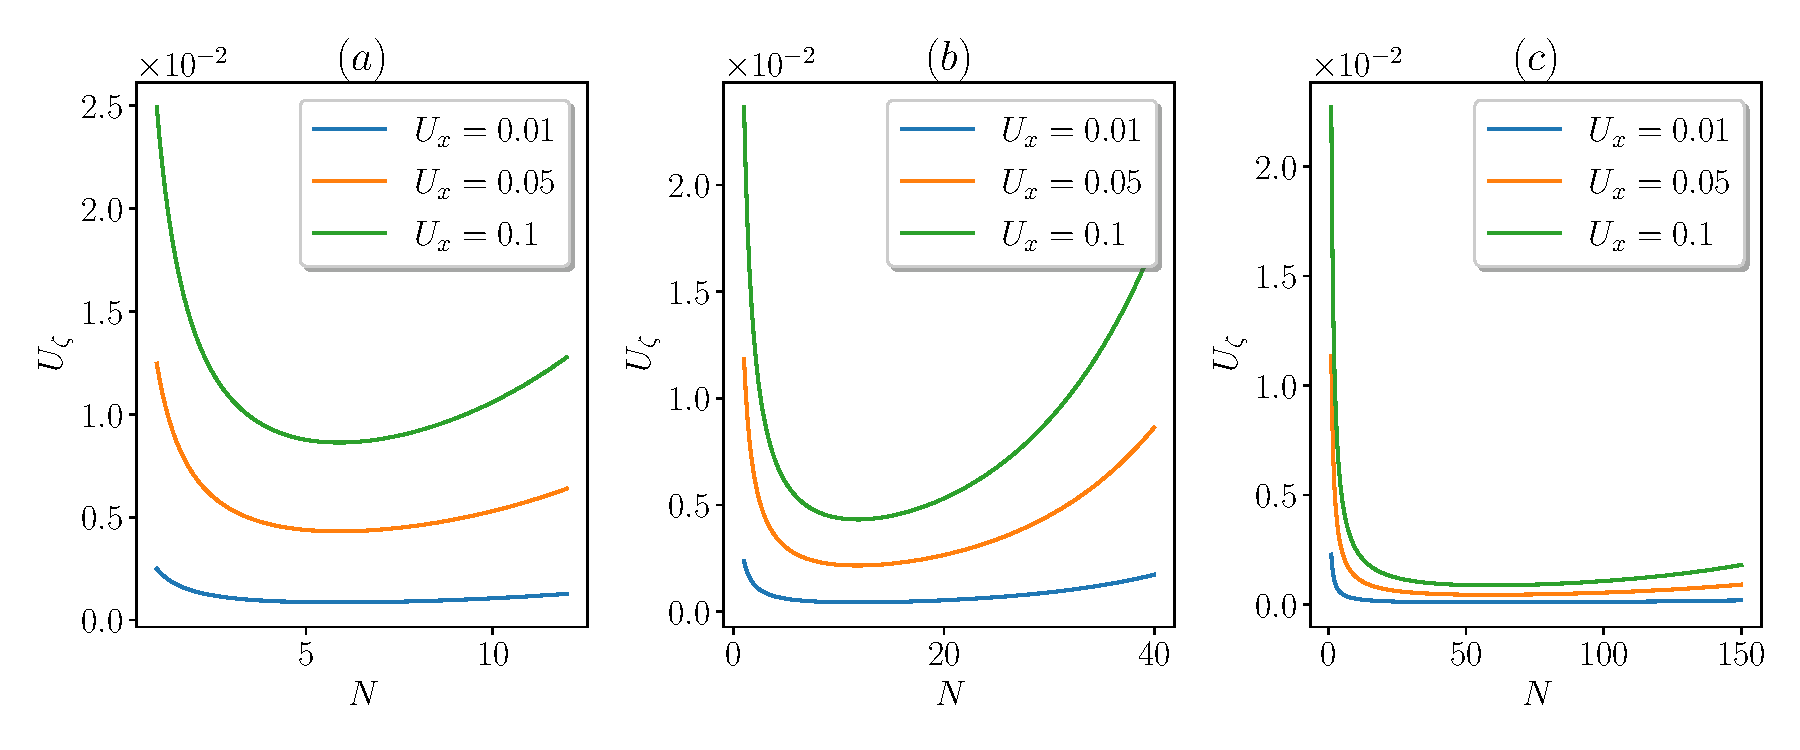
\includegraphics[scale=0.55]{fig1}
\centering
\caption{The variation of uncertainty $U_\xi$ with respect to  number of periods $N$ for various damping ratios($\xi$). (a) $\xi$ = 0.030, (b)$\xi$= 0.015, and (c)$\xi$ = 0.003.}
\label{f1}


\end{figure*}
Fig.~\ref{f1} shows the variation of uncertainty $U_\xi$ with respect to $N$ number of periods for various damping ratios($\xi$). (a) $\xi$ = 0.030, (b)$\xi$= 0.015, and (c)$\xi$ = 0.003.

 The optimal number of periods $N$ is obtained by differentiating $U_\xi$ with respect $N$ and solving for $N$, which is
\begin{figure}[h]


\centering

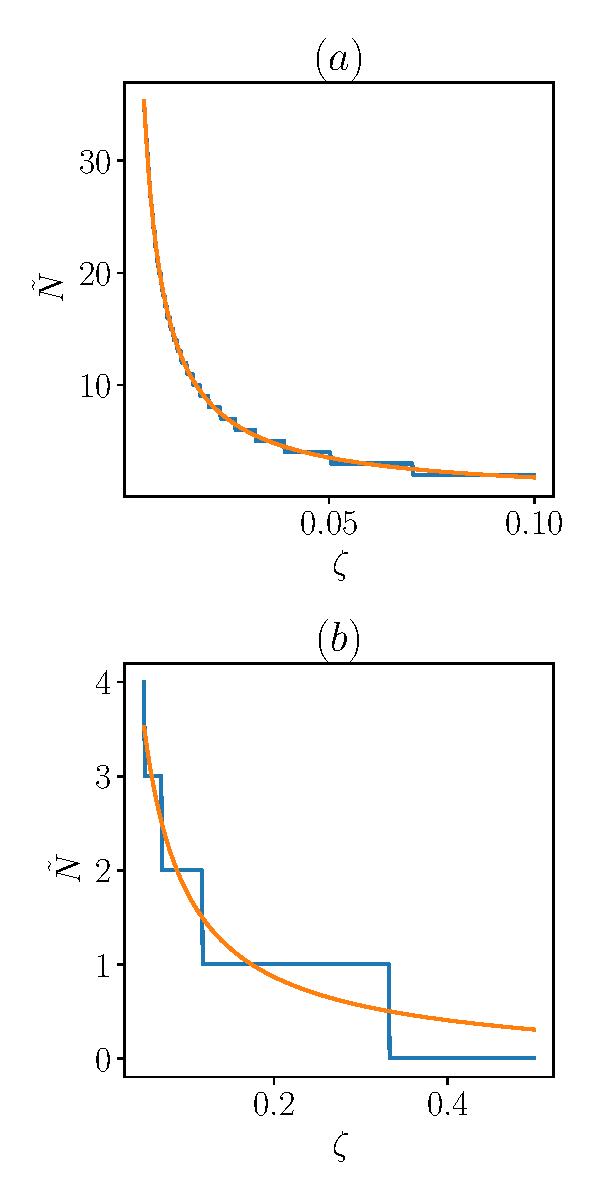
\includegraphics[scale=0.6]{fig3}
\caption{The optimal number of periods $N$ for predicting accurate damping ratios $\xi$ }
\label{f2}
\end{figure}

\begin{equation}
N_{\rm{opt}}=\frac{1}{4} \frac{\left(2+\mathrm{W}\left(2 \mathrm{e}^{-2}\right)\right) \sqrt{-(\xi-1)(\xi+1)}}{\pi \xi}.
\end{equation}
From Fig.~\ref{f2} we observe that uncertainty analysis gives us the optimum number of periods for damping ratios($\xi$) up to $0.1$. 
As the damping ratio increases beyond $0.1 $, we will be unable to determine the optimal number of periods.
%%%%%%%%%%%%%%%%%%%%%%%%%%%%%%%%%%%%%%%%%%%%%%%%%%%%%%%%%%%%%%%%%%%%%%
%!TEX root = ..\arxiv_Dampinguncertanity_manuscript.tex
%-------------------------------
%*******************************
\section{UNCERTAINTY ANALYSIS}
\label{sec:method}

In this section, we perform the uncertainty analysis on the areas approach~\cite{Huang2007} to identify the structural damping ratio. 
We develop guidelines for an optimal number of areas to be considered for accurate damping estimation. This method yields precise estimate of the damping ratio with noise, even for a higher damping ratio($\xi$).

We define the areas logarithmic decrement ratio as
\begin{equation}
\delta_{\rm A}=\ln \frac{A_{1}}{A_{n+1}}=\ln \frac{A \mathrm{e}^{-\xi \omega_{n} t_{i}}}{A \mathrm{e}^{-\xi \omega_{n}\left(t_{i}+n T_{d}\right)}}=\xi \omega_{n} T_{d} n=\frac{2 n \pi \xi}{\sqrt{1-\xi^{2}}},
\end{equation}
where $T_d$ is damped time period, $\omega_{n}$ is the natural frequency, $n$ number of periods and $A$ is the amplitude of the signal.
\begin{figure}[h]
\label{sin}
\includegraphics[scale=0.25]{sinwave_area}
\centering
\caption{The free decay response of the signal.}
\end{figure}

Next, we define $S_{1}, \ldots, S_{N}$ (see Fig.~\ref{sin}) as the areas corresponding to the zero-crossings of the signal. 
For example, the expressions for the two first areas are given by 
\begin{equation}
\label{e9}
\begin{aligned}
&S_{1}=\int_{t_{1}}^{t_{1}+\frac{T_{d}}{2}}|x(t)| \mathrm{d} t=\int_{0}^{\frac{T_{d}}{2}}\left|x\left(t+t_{1}\right)\right| \mathrm{d} t\\
&=A \mathrm{e}^{-\xi \omega_{n} t_{1}} \int_{0}^{\frac{T_{d}}{2}}\left|\mathrm{e}^{-\xi \omega_{n} t} \sin \left(\omega_{d} t+\varphi+\omega_{d} t_{1}\right)\right| \mathrm{d} t\\
&S_{2}=\int_{t_{1}+\frac{T_{d}}{2}}^{t_{1}+T_{d}}|x(t)| \mathrm{d} t=\int_{0}^{\frac{T_{d}}{2}}\left|x\left(t+t_{1}+\frac{T_{d}}{2}\right)\right| \mathrm{d} t\\
&=A \mathrm{e}^{-\xi \omega_{n} t_{1}} \mathrm{e}^{-\xi \omega_{n} \frac{T_{d}}{2}} \int_{0}^{\frac{T_{d}}{2}}\left|\mathrm{e}^{-\xi \omega_{n} t} \sin \left(\omega_{d} t+\varphi+\omega_{d} t_{1}\right)\right| \mathrm{d} t.
\end{aligned}
\end{equation}

The relationship between areas can be obtained from Eq.~\eqref{e9} as
\begin{equation}
\label{e1}
S_{2}=S_{1} \mathrm{e}^{-\xi \omega_{n} \frac{T_{d}}{2}}.
\end{equation}
Similarly one can obtain
\begin{equation}
\label{e2}
S_{2 N}=S_{2 N-1} \mathrm{e}^{-\xi \omega_{n} \frac{T_{d}}{2}}.
\end{equation}
The expression for $\xi$ in terms of $S_{1}..S_{N}$, can be obtained as follows
\begin{equation}
\label{eq1}
\begin{aligned}
&\frac{S_{1}+S_{2}+\cdots+S_{N}}{S_{N+1}+S_{N+2}+\cdots+S_{2 N}}=\frac{S_{1}+S_{2}+\cdots+S_{N}}{\left(S_{1}+S_{2}+\cdots+S_{N}\right) \mathrm{e}^{-\xi \omega_{n} n T_{d}/2}}\\ &=\mathrm{e}^{\xi \omega_{n} n T_{d}/2}=\mathrm{e}^{ n \pi \xi} / \sqrt{1-\xi^{2}}.
\end{aligned}
\end{equation}
From Eq.~\eqref{eq1} damping ratio $\xi$ is
\begin{equation}
\xi=1 / \sqrt{1+\left(n \frac{\pi}{E}\right)^{2}},
\end{equation}
where $E=\ln \left(\sum S_{k} / \sum S_{k+N}\right)$, which is the natural logarithm of the ratio of summation of the former $N$ areas to the summation of the latter $N$ areas.


From equations Eqs.\eqref{e1} and \eqref{e2} we can write

\begin{equation}
\begin{array}{c}

S_{2}=S_{1}\epsilon\\
S_{3}=S_{1} \epsilon^{2} \\
\vdots \\
S_{N}=S_{1} \epsilon^{N-1}
\end{array}
\end{equation}
where $ \epsilon=\mathrm{e}^{-\xi \omega_{n} \frac{T_{d}}{2}}.$

The summation of first $N$ areas in Eq.~\eqref{eq1} is given by
\begin{equation}
\begin{aligned}
U_N=S_{1}+S_{2}+\cdots+S_{N}=S_1 (1+\epsilon+\epsilon^2+\epsilon^3\cdots\epsilon^{N-1}).
\end{aligned}
\end{equation}
Differentiating $U_N$ with respect to $\xi$ gives
% \begin{equation}
\begin{align}
\frac{\partial U_N}{\partial \xi}&=S_{1}(0+c\epsilon+2c\epsilon^2+3c\epsilon^3\cdots(N-1)c\epsilon^{N-1}), \nonumber\\
                                 &=S_{1}c\epsilon(1+2\epsilon+3\epsilon^2+\cdots+(N-1)\epsilon^{N-2})  
\label{e3}
\end{align}
% \end{equation}

% \begin{equation}
% \label{e3}
% \frac{\partial U_N}{\partial \xi}=S_{1}c\epsilon(1+2\epsilon+3\epsilon^2\cdots(N-1)\epsilon^{N-2}),
% \end{equation}
where $c=-\omega_{n} \frac{T_{d}}{2}$.\\
Eq.~\eqref{e3} is an arithmetic geometric progression, with $\mid \epsilon \mid \leq 1 $. 
The sum of terms of the progression is given by
\begin{equation}
\label{e6}
\frac{\partial U_N}{\partial \xi}=S_{1}c\epsilon\left[\frac{1-N \epsilon^{N-1}}{1-\epsilon}+\frac{\epsilon \left(1-\epsilon^{N-1}\right)}{(1-\epsilon)^{2}}\right].
\end{equation}
Similarly, we can write the summation of the subsequent $N$ areas in Eq.\eqref{eq1} as
\begin{equation}
\begin{aligned}
U_D&=S_{N+1}+S_{N+2}+\cdots+S_{2N}\\
&=S_1 \epsilon^N(1+\epsilon+\epsilon^2+\epsilon^3\cdots\epsilon^{N-1}).
\end{aligned}
\end{equation}
Differentiating $U_D$ with respect to $\xi$ gives
\begin{multline}
\label{e7}
\frac{\partial U_D}{\partial \xi}=S_{1}N c \epsilon^N(1+\epsilon+\epsilon^2+\epsilon^3\cdots\epsilon^{N-1})\\
+S_1 \epsilon^N(0+c\epsilon+2c\epsilon^2+3c\epsilon^3\cdots(N-1)c\epsilon^{N-1}).
\end{multline}

In Eq.~\eqref{e7}, we notice that the first term is a geometric series, and the second term is an arithmetic geometric progression with $\mid \epsilon \mid \leq 1 $. 
The sum of the terms then becomes
\begin{multline}
\label{equd}
\frac{\partial U_D}{\partial \xi}=S_{1}N c \epsilon^N \left(\frac{1-\epsilon^{N}}{1-\epsilon}\right)\\
+S_1c \epsilon^{N+1}\left[\frac{1-N \epsilon^{N-1}}{1-\epsilon}+\frac{\epsilon \left(1-\epsilon^{N-1}\right)}{(1-\epsilon)^{2}}\right].
\end{multline}

The total uncertainty in Eq.\eqref{eq1} is given by
\begin{equation}
\label{equn}
U^2_{\xi}=\left[\left(\frac{\partial U_{N}}{\partial \xi}\right)^{2}+\left(\frac{\partial U_{D}}{\partial \xi}\right)^{2}\right]U_x^2,
\end{equation}
where $U_x$ is the uncertainty in measuring the response. 
Substituting Eqs.~\eqref{e6}~and~\eqref{equd} into Eq.~\eqref{equn} gives
\begin{equation}
\label{tuc}
\begin{array}{l}
U_{\xi}^{2}=\left\{\left(S_{1} c \varepsilon\left[\frac{1-N \varepsilon^{N-1}}{1-\varepsilon}+\frac{\varepsilon\left(1-\varepsilon^{N-1}\right)}{(1-\varepsilon)^{2}}\right]\right)^{2}\right. \\
\left.+\left(S_{1} N c \varepsilon^{N}\left(\frac{1-\varepsilon^{N}}{1-\varepsilon}\right)+S_{1} c \varepsilon^{N+1}\left[\frac{1-N \varepsilon^{N-1}}{1-\varepsilon}+\frac{\varepsilon\left(1-\varepsilon^{N-1}\right)}{(1-\varepsilon)^{2}}\right]\right)^{2}\right\}U_x^2
\end{array}
\end{equation}

\begin{figure}[h]

\centering
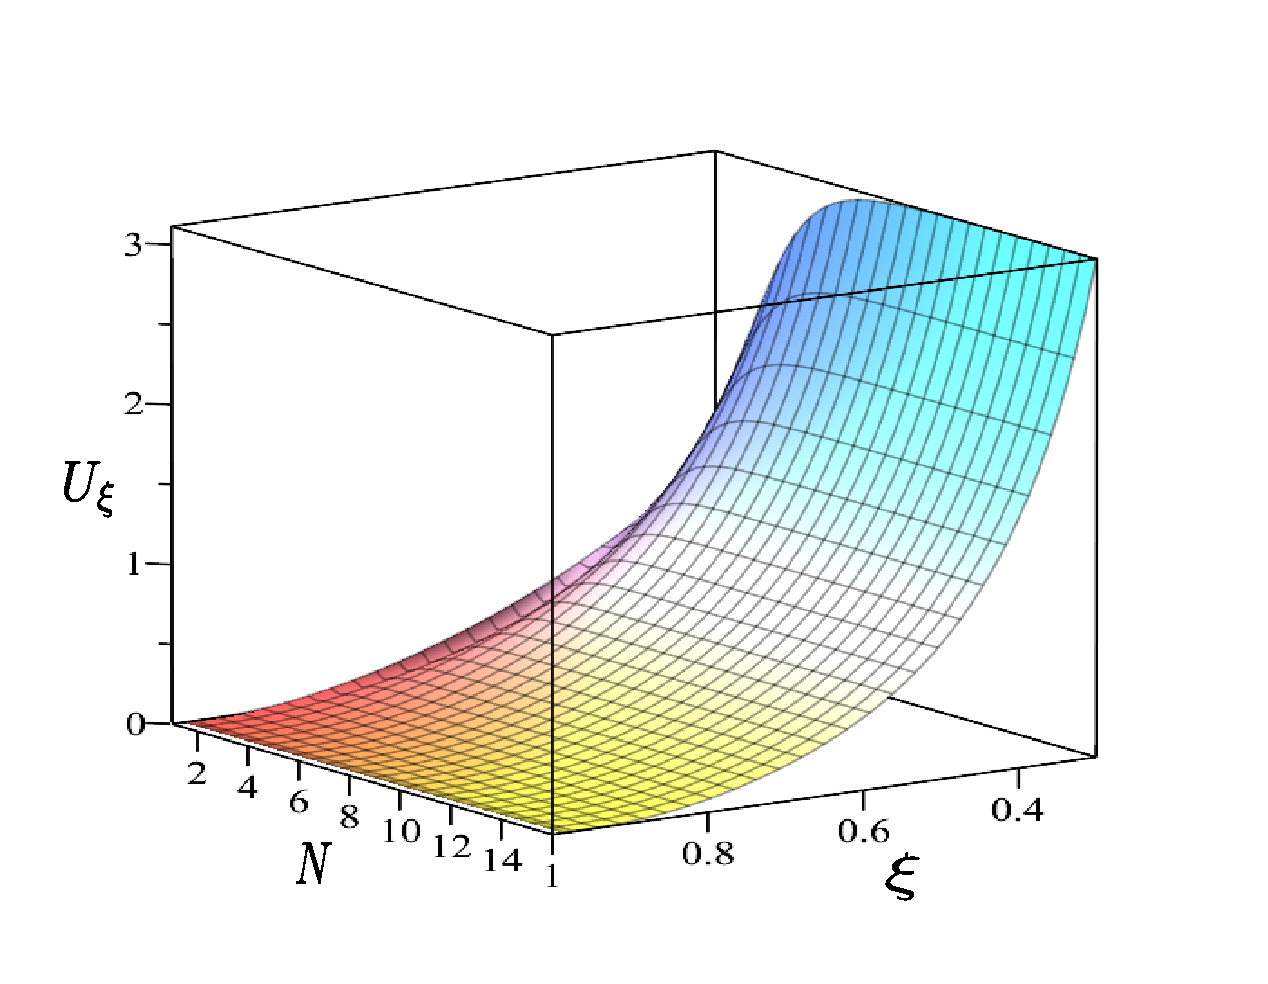
\includegraphics[scale=0.45]{Surf1uz0p3}

\caption{The variation of uncertainty ($U_{\xi}$) with $N$ and $\xi$.}
\label{4}


\end{figure}

Figure~\ref{4} shows the uncertainty $U_{\xi}$ variation with $N$ and $\xi$, we can observe that as $\xi$ decreases and $N$ increases, the uncertainty will be maximum.

Our goal is to find out the optimal number of areas to minimize the uncertainty in predicted damping ratio $\xi$. Which can be achieved by differentiating $U_\xi$ with respect $N$ and solving for $N$.
Differentiating Eq.~\eqref{tuc} with respect to $N$ yields
\begin{equation}
\label{e10}
\begin{aligned}
&\frac{\partial U_{\xi}}{\partial N}=\left\{2 S_1^{2} c^{2} \epsilon^{2}\left(\frac{1-N \epsilon^{N-1}}{1-\epsilon}+\frac{\epsilon\left(1-\epsilon^{N-1}\right)}{(1-\epsilon)^{2}}\right)\right. \\
&\left(\frac{-\epsilon^{N-1}-N \epsilon^{N-1} \ln (\epsilon)}{1-\epsilon}-\frac{\epsilon \epsilon^{N-1} \ln (\epsilon)}{(1-\epsilon)^{2}}\right)\\
&+2\left(\frac{S_1 N c \epsilon^{N}\left(1-\epsilon^{N}\right)}{1-\epsilon}+S_1 c \epsilon^{N+1}\left(\frac{1-N \epsilon^{N-1}}{1-\epsilon}+\frac{\epsilon\left(1-\epsilon^{N-1}\right)}{(1-\epsilon)^{2}}\right)\right) \\
&\left(\frac{S_1 c \epsilon^{N}\left(1-\epsilon^{N}\right)}{1-\epsilon}+\frac{S_1 N c \epsilon^{N} \ln (\epsilon)\left(1-\epsilon^{N}\right)}{1-\epsilon}-\frac{S_1 N c\left(\epsilon^{N}\right)^{2} \ln (\epsilon)}{1-\epsilon}\right. \\
&\left.+S_1 c \epsilon^{N+1} \ln (\epsilon)\left(\frac{1-N \epsilon^{N-1}}{1-\epsilon}+\frac{\epsilon\left(1-\epsilon^{N-1}\right)}{(1-\epsilon)^{2}}\right)\right. \\
&\left.+S_1 c \epsilon^{N+1}\left(\frac{-\epsilon^{N-1}-N \epsilon^{N-1} \ln (\epsilon)}{1-\epsilon}-\frac{\epsilon \epsilon^{N-1} \ln (\epsilon)}{(1-\epsilon)^{2}}\right)\right\}\frac{ U_{x}}{2U_{\xi}}.
\end{aligned}
\end{equation}

Equation~\eqref{e10} does not have have a closed form solution for $N \geq 2$; therefore, we must use numerical solutions to obtain the optimal $N$. 
Note that we assume that $S_1=1$, i.e., we do not consider uncertainties in the zero-crossings in our analysis. The uncertainty in measurement($U_x$) will not affect the optimal number areas since it is constant.
\begin{figure}[h]
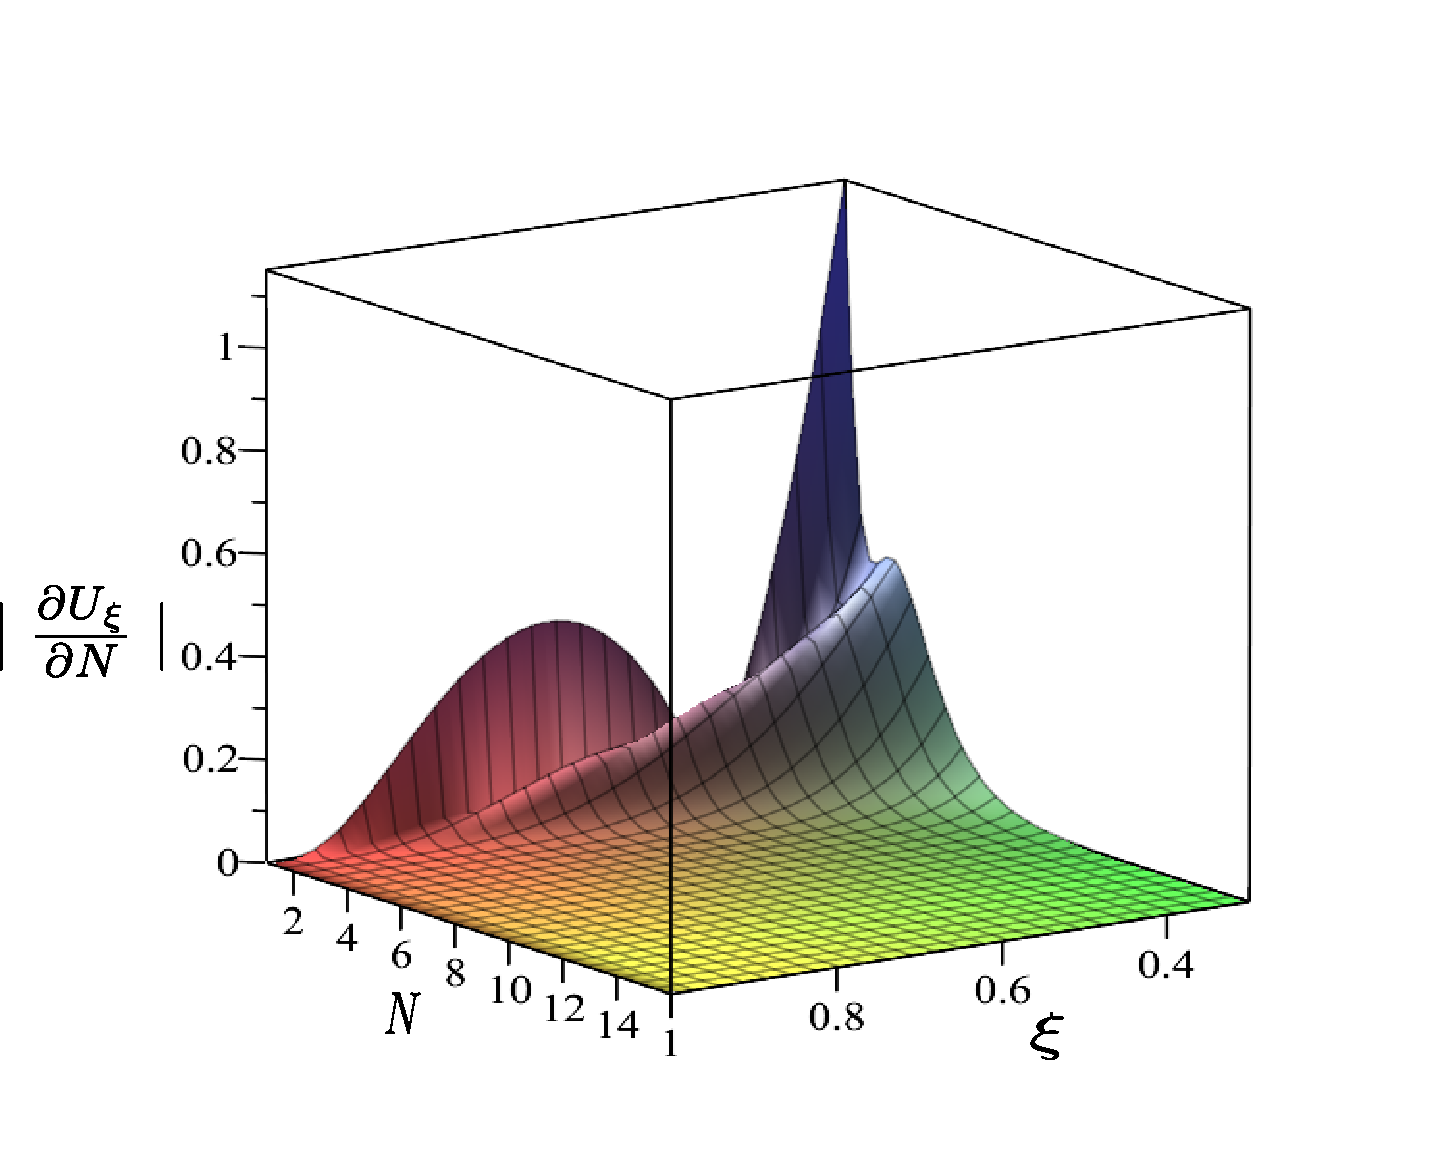
\includegraphics[scale=0.4]{Surf1z0p3}
\centering
\caption{The variation of rate of uncertainty with $N$ for high damping ratio($\xi$).}
\label{uH}
\end{figure}
\begin{figure}[h]
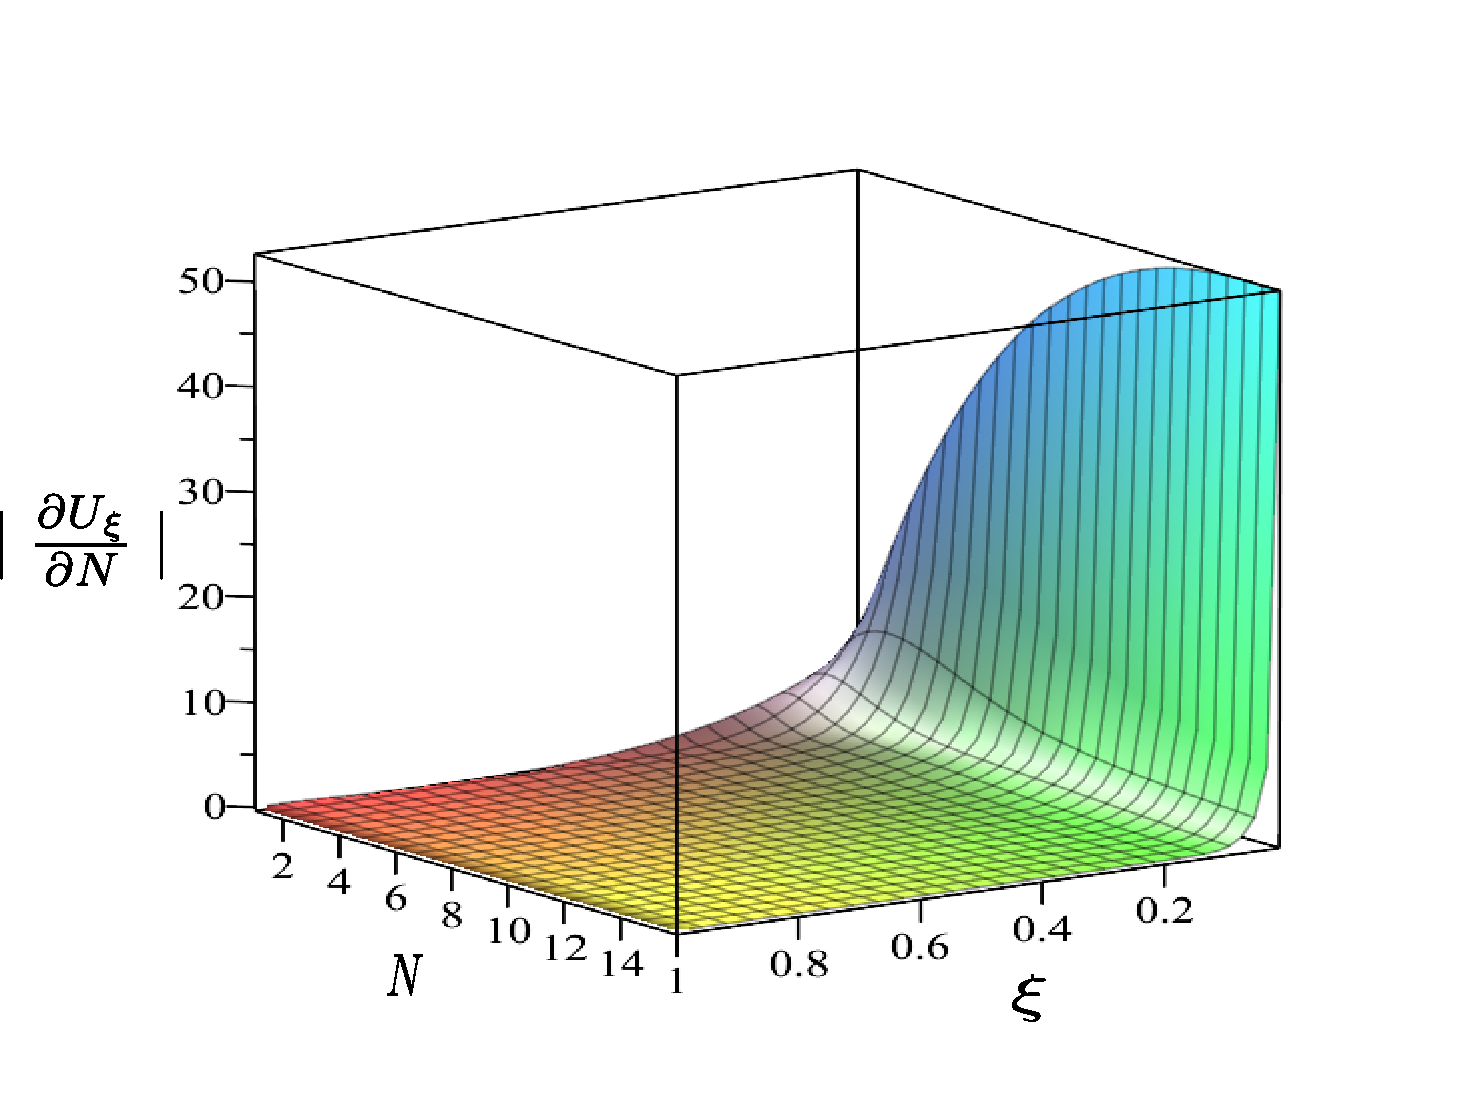
\includegraphics[scale=0.4]{Surf1z0p1}
\centering
\caption{The variation of rate of uncertainty with $N$ and for low to high damping ratio($\xi$).}
\label{uL}
\end{figure}

\begin{figure}[h]
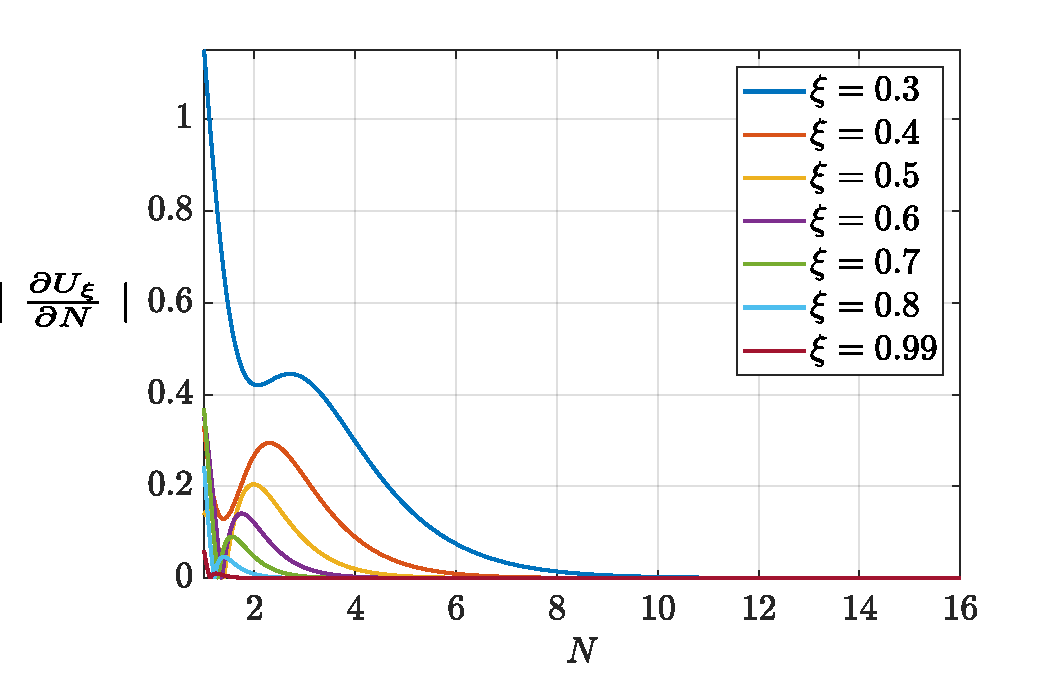
\includegraphics[scale=0.5]{zN}
\centering
\caption{The variation of rate of uncertainty with $N$ for high damping ratio($\xi$).}
\label{uH1}
\end{figure}
\begin{figure}[h]
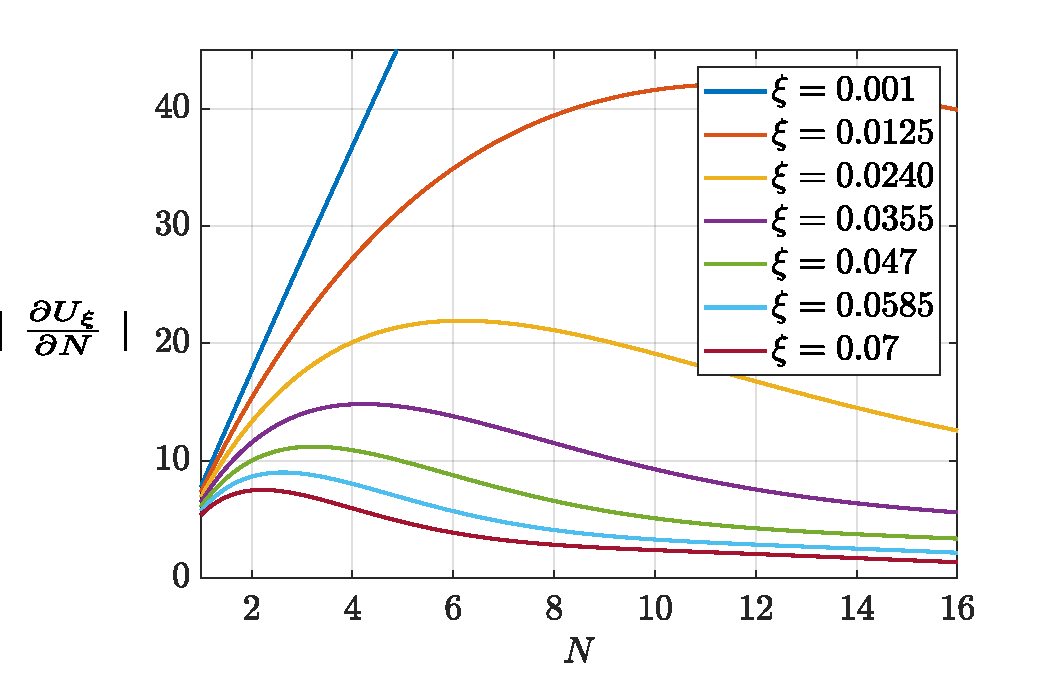
\includegraphics[scale=0.5]{zN1}
\centering
\caption{The variation of rate of uncertainty with $N$ for very low damping ratio($\xi$).}
\label{uL1}
\end{figure}

From Figs.~\ref{uH} and \ref{uH1}, we can observe that for high damping ratios, we see a local maximum in the rate of uncertainty with N. We can also observe that the uncertainty decreases as $N$ increases. Based on these observations, we can say that for a high damping ratio $\xi$, consider as many areas as possible and avoid picking up $N$, which is at local maxima to minimize the error in predicted $\xi$.
For a very low damping ratio, from Fig.~\ref{uL1} we can see that the rate of uncertainty increases enormously as we raise $N$ for very low damping we need to consider as minimum areas as possible to minimize the error in predicted $\xi$.
%%%%%%%%%%%%%%%%
%%%%%%%%%%%%%%%%


%%%%%%%%%%%%%%%%%%%%%%%%%%%%%%%%%%%%%%%%%%%%%%%%%%%%%%%%%%%%%%%%%%%%%%
%!TEX root = ..\arxiv_Dampinguncertanity_manuscript.tex
%-------------------------------
%*******************************
\section{NUMERICAL EXPERIMENTS}
\label{sec:results}
%*******************************
In this section, we perform a large number of numerical experiments to verify our results. 
We consider a single degree of freedom oscillator as
\begin{equation}
\ddot{x}+0.5 \dot{x}+25 x=0
\end{equation}

The system response is given by
\begin{equation}
x(t)=\mathrm{e}^{-0.25 t} \sin \left(\omega_{d} t+\varphi\right)
\end{equation}
where $\omega_{d}=\omega_{n} \sqrt{1-\xi^{2}}, \varphi=\arctan 10$, $\omega_{n}=5$, $\xi=0.05$ and $x(t)$ is displacement.
\begin{figure}[h]
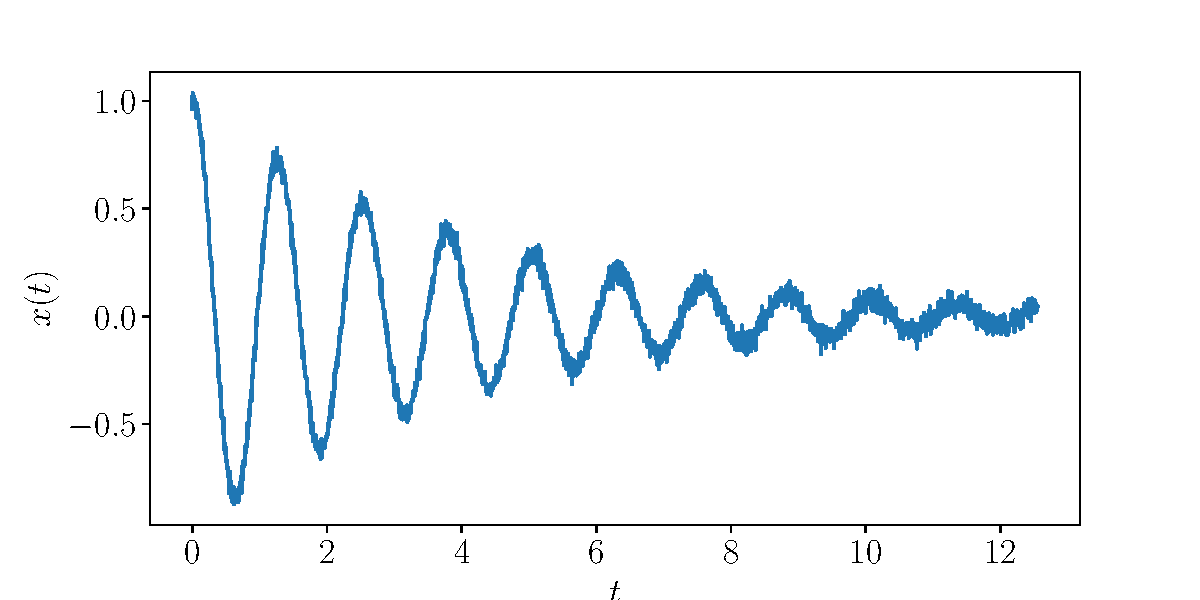
\includegraphics[scale=0.5]{nwave}
\label{f4}
\centering
\caption{The response $x(t)$ with  Gaussian noise of SNR 20.}
\end{figure}
\begin{figure}[ht]
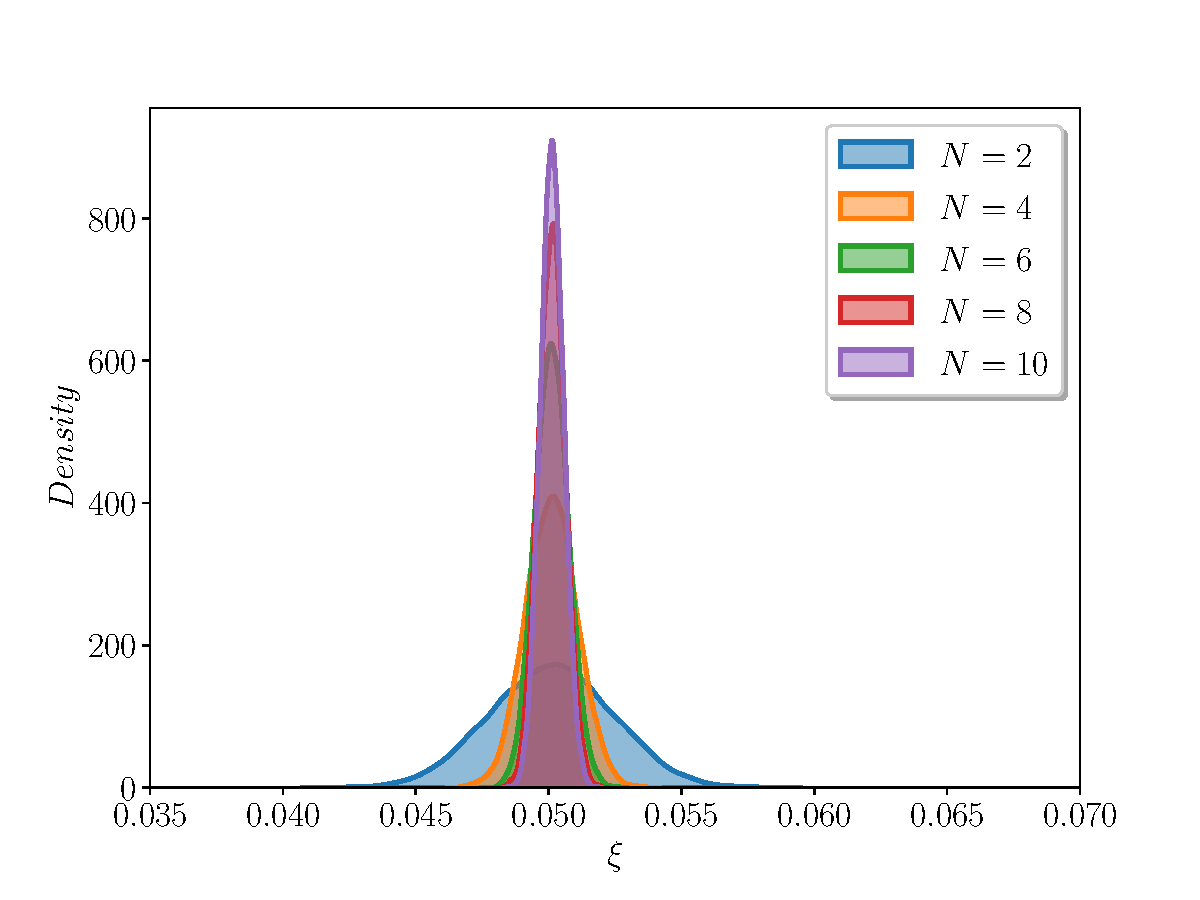
\includegraphics[scale=0.5]{fig5_1}
\label{f4}
\centering
\caption{The distribution of $\xi$ with 10000 times simulated for Gaussian noise of SNR 20 and with N.}
\end{figure}

\begin{figure}[h]
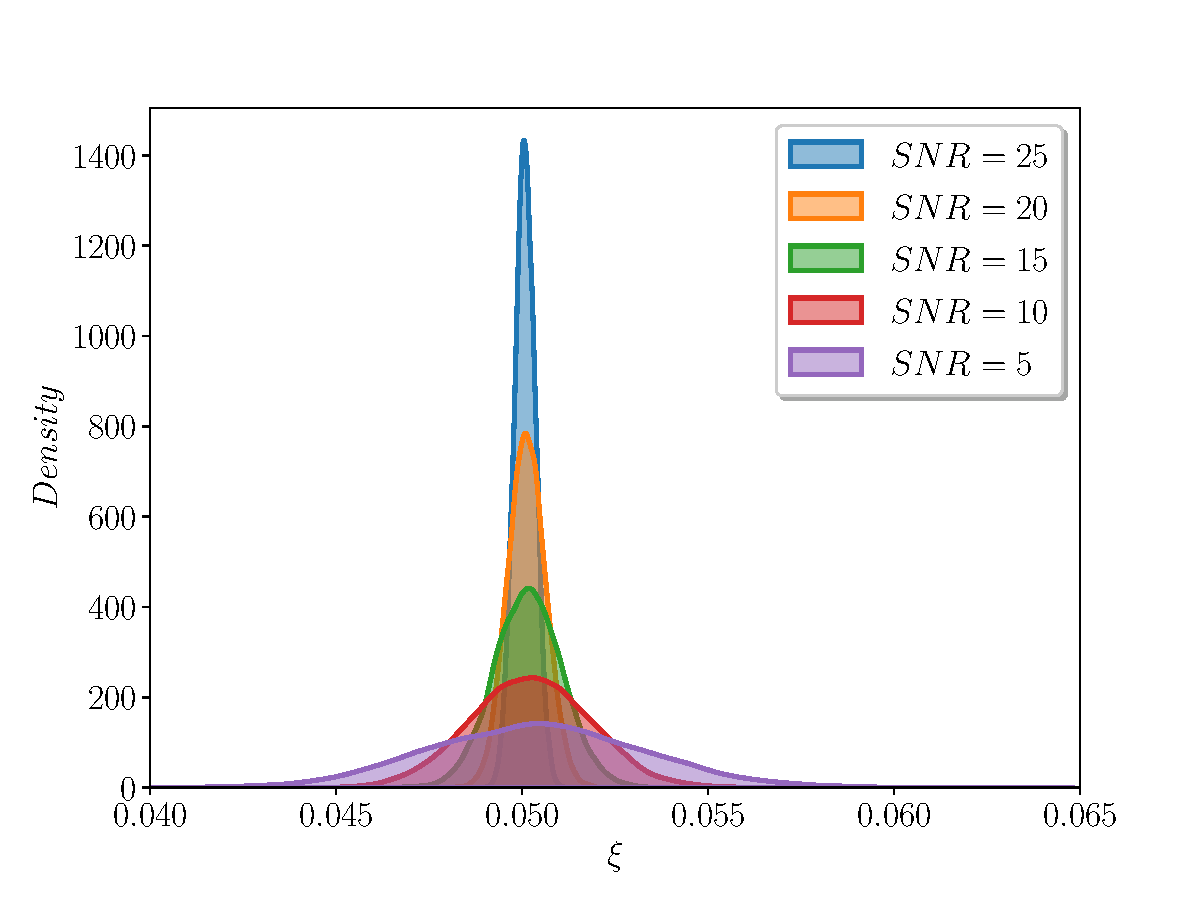
\includegraphics[scale=0.5]{fig_snrv}
\centering
\caption{The distribution of $\xi$ with 10000 times simulated for N=8 and with SNR.}
\end{figure}

From Fig.~\ref{f4} we observe that as we increase the number of areas, the error in the predicted $\xi$
becomes small after a certain number of areas, the increment in areas will not benefit much. 
This jives with our observations from the uncertainty analysis results in Fig.~\ref{uL1}. 
We also observe that as the noise increases, our prediction accuracy in $\xi$ decreases, which is expected, but the error in this analysis is less than the same system studies in ~\cite{Huang2007}. 
%%%%%%%%%%%%%%%%%%%%%%%%%%%%%%%%%%%%%%%%%%%%%%%%%%%%%%%%%%%%%%%%%%%%%%
%!TEX root = ..\arxiv_Dampinguncertanity_manuscript.tex
%-------------------------------
%*******************************
\section{CONCLUSION}
\label{sec:conclusion}
%*******************************
This study findings provide guidelines for choosing the optimal number of areas to be considered in the area ratio damping estimation method. The area ratio damping gives a better estimation of damping in high damping and noisy environments than the logarithmic decrement method. We developed guidelines to make the area ratio damping method for more robust damping estimation. We are not aware of any prior studies for finding the optimal number of areas in the area ratio damping estimation method.

The uncertainty analysis performed in this work gives more insights into choosing the optimal number of areas. Our guidelines suggest that for a very low damping ratio ($<0.01$), choosing more than two areas in the estimation increases the uncertainty.
In contrast, for moderate to high damping (between $0.05$ and $1$), we need to consider all the available areas in the estimation.

When we consider the uncertainties in zero-crossings, the analysis becomes significantly complicated. Therefore we have not included uncertainties in zero-crossings. We left the uncertainty analysis with considering zero-crossings  as future work.
%%%%%%%%%%%%%%%%%%%%%%%%%%%%%%%%%%%%%%%%%%%%%%%%%%%%%%%%%%%%%%%%%%%%%%
\section*{ACKNOWLEDGMENTS}
\label{sec:acknowledgments}
% %*******************************
This material is based upon work supported by the National Science Foundation under grants CMMI-1759823 and DMS1759824. Trial 123457677pko6
\newpage
\bibliographystyle{plain}
\bibliography{bib}

\end{document}
